\chapter*{Inleiding}
\markboth{Inleiding}{Inleiding}

De {\fontseries{extrabold}\selectfont Cryptomanual}   \say{{\fontseries{medium}\selectfont Best Practices}} is een uitstekende plek om te beginnen met Bitcoin, blockchain en cryptocurrencies. Indien je niet maandenlang bezig wilt zijn met onderzoek naar de basisbeginselen van deze technologie en de impact er van, dan kun je met onze manual snel en makkelijk van start gaan. Alles samen hebben wij meer dan 6 jaar onderzoek in onze digitale handleidingen (e-manuals) gestopt en ons doel is om \emph{beginnen met cryptocurrencies} voor iedereen zo laagdrempelig mogelijk te maken. \medskip 
\noindent Al ons materiaal is gemakkelijk te navigeren en heeft als doel jou te helpen de basis onder de knie te krijgen. Daarnaast zorgen wij ervoor dat je valkuilen en misvattingen vermijdt terwijl je over geld, cryptocurrencies, relevante technologie{\"e}n en de implicaties ervan leert. Tussendoor vind je allerlei \emph{Tips} en \emph{Tops}, waar je direct mee aan de slag kunt. De e-manual kan van a tot z worden bestudeerd, maar elk onderdeel staat ook op zich. \medskip 

\begin{figure}[ht!]
    \centering
    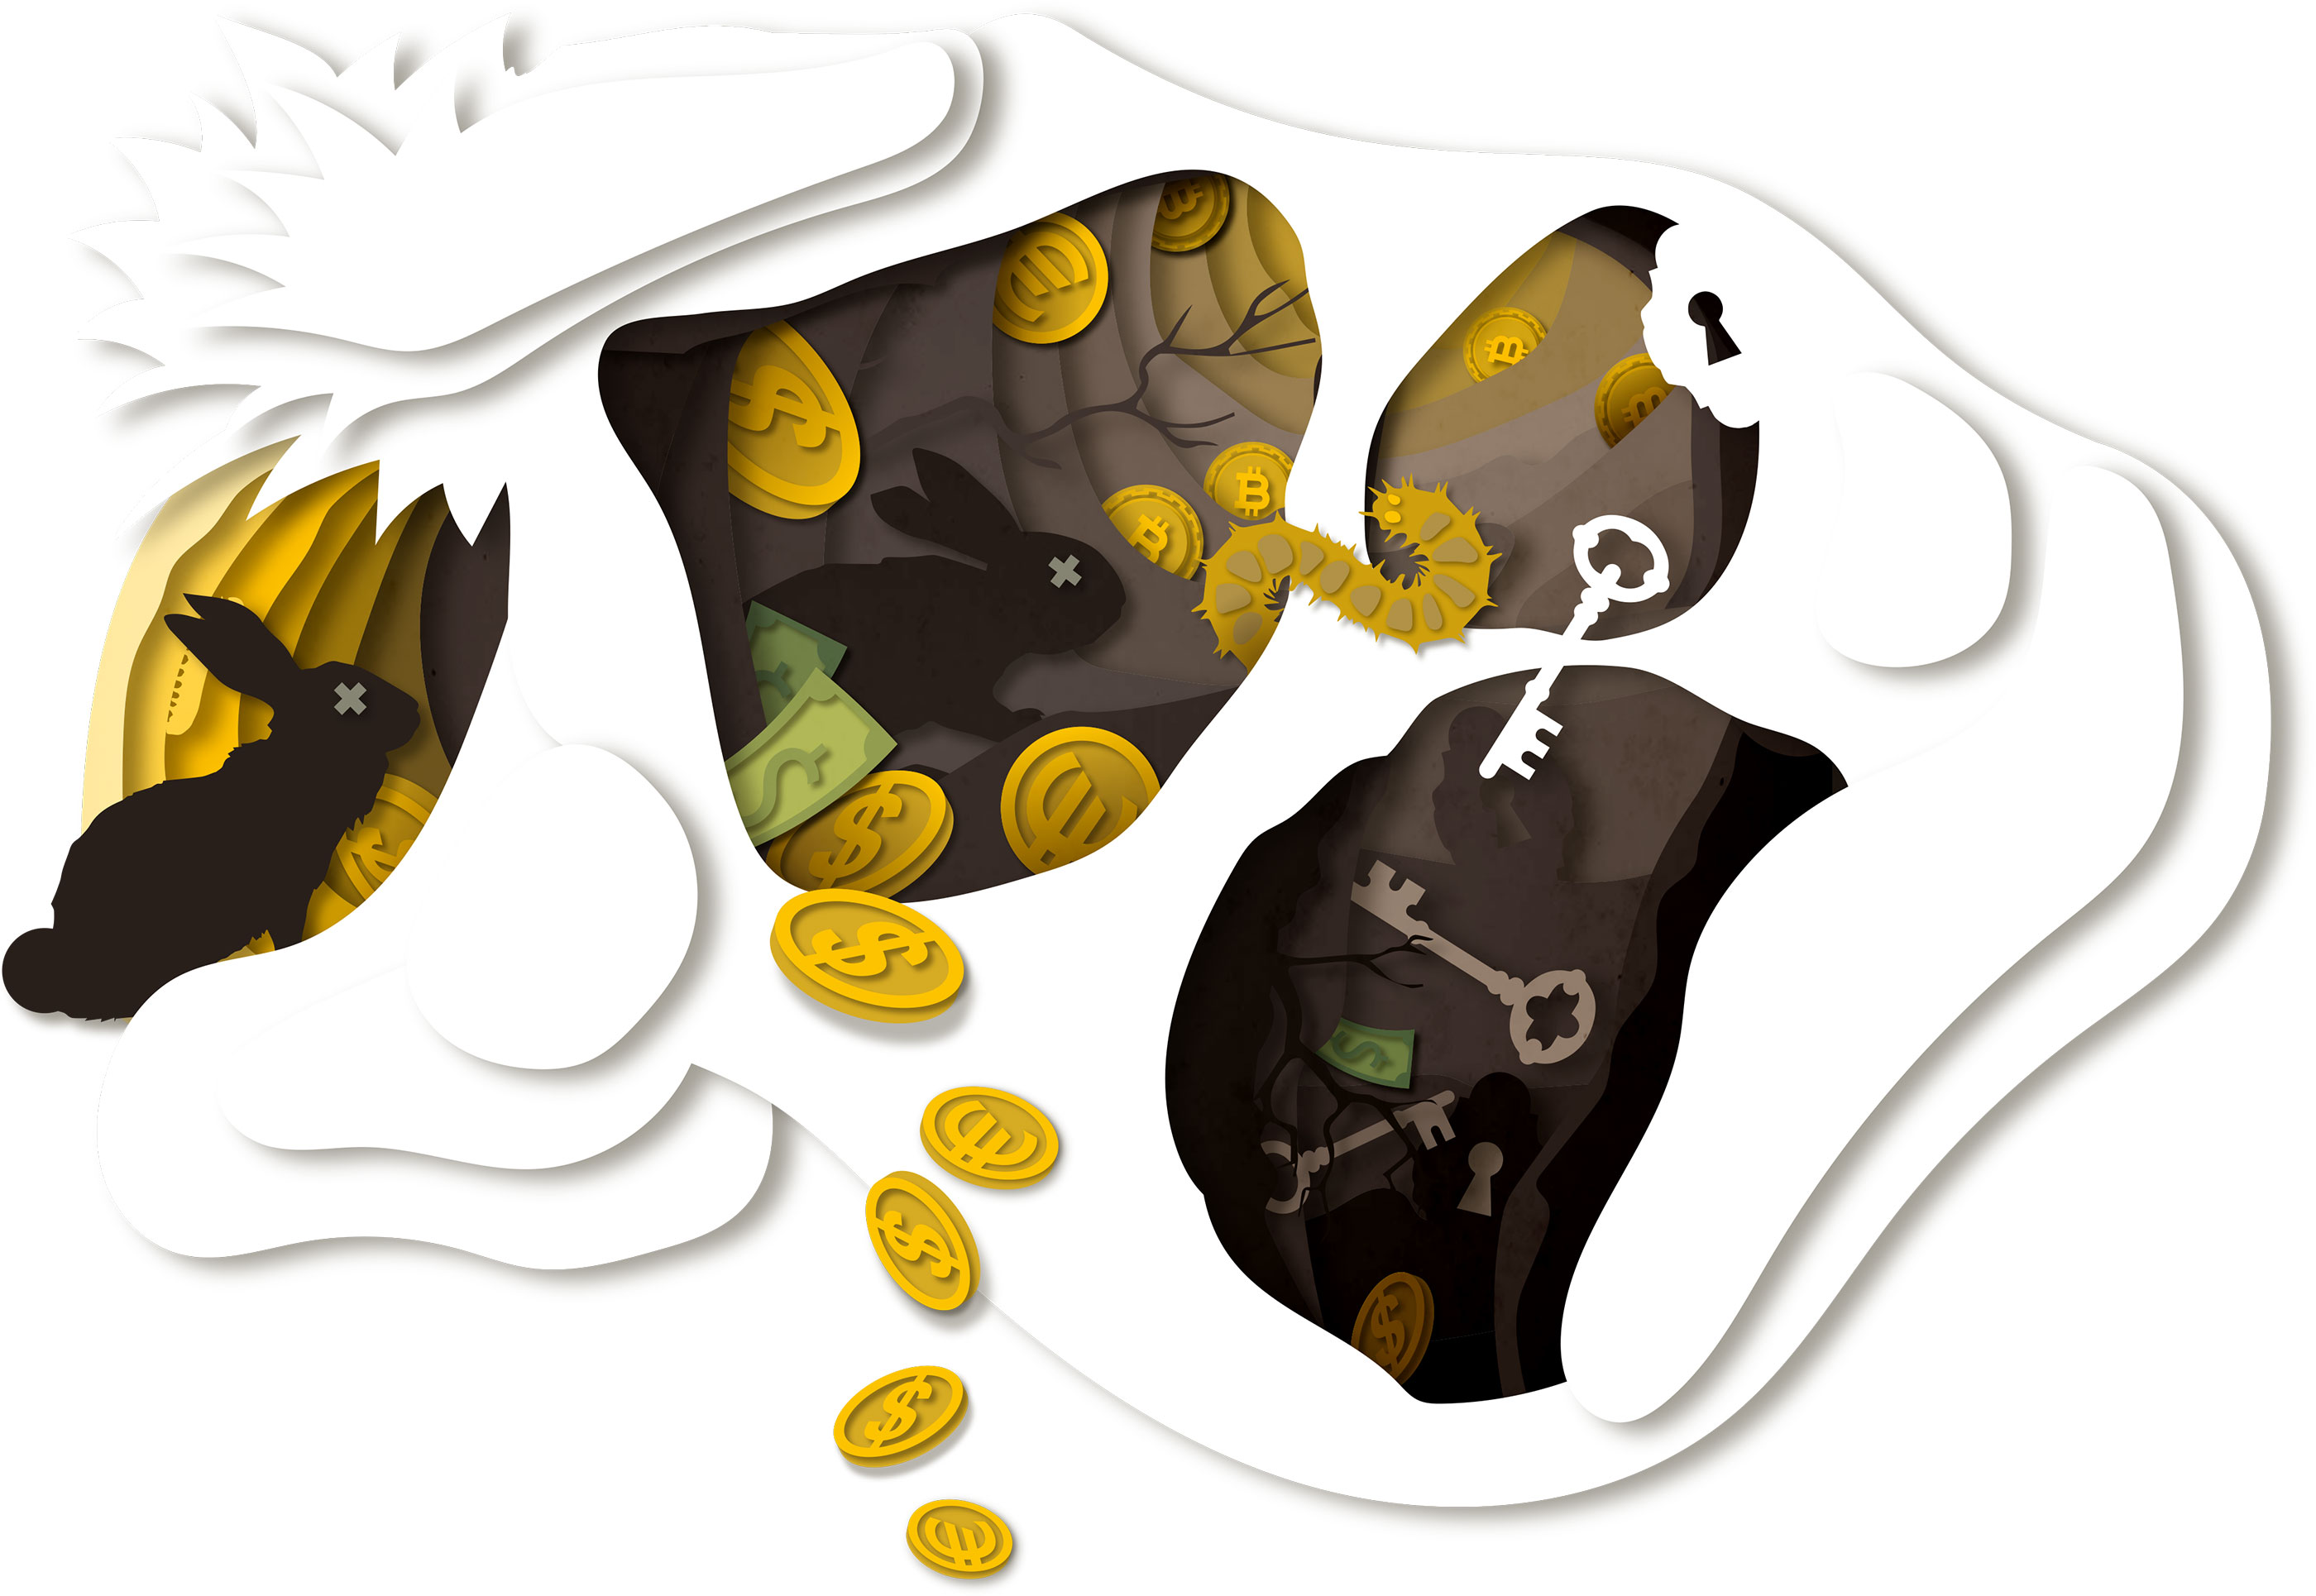
\includegraphics[width=\textwidth]{illustrations/resized_CRYPTO_KEY_1_PART_1.jpg}
\end{figure}

\medskip

De Cryptomanual behandelt een aantal van de meest belangrijke en noodzakelijke topics omtrent wallets \& exchanges en biedt hulpmiddelen en informatie met betrekking tot het kopen, bewaren en verhandelen van cryptocurrencies. Proficiat, je hebt de eerste stap gezet en maakt nu deel uit van de baanbrekende cryptocurrency-revolutie. We staan aan het begin van een nieuwe fase van het digitale tijdperk: \emph{the internet of value}.\medskip 

\begin{tipbox}{Tip}
Ga voor een selectie van top video's naar  \href{https://cryptomanuals.com/5-videos-to-start-with-bitcoin}{cryptomanuals} om te leren over Bitcoin, crypto en het geldsysteem.
\end{tipbox}


\section*{Internet of Value}
De eerste golf van digitalisering bracht ons \emph{the internet of information}. De tweede golf brengt ons \emph{the internet of value}. The internet of value is een nieuw, gedistribueerd platform dat een nieuwe rol gaat spelen bovenop de huidige internet infrastructuur. Het helpt ons om de digitale wereld en het bedrijfsleven zoals wij deze kennen opnieuw vorm te geven en de oude orde van de mensheid ten goede te transformeren. Veelal zullen deze ontwikkelingen zich eerst achter de schermen afspelen en mede daardoor is de impact ervan niet direct voor iedereen zichtbaar. 

\bigskip
 
\begin{cryptobox}{THIS TIME IT'S GLOBAL}
  
\textit{Deze tweede fase van de digitale [r]evolutie stelt mensen in staat om geld en andere activa te verplaatsen over het internet, zoals mensen al decennia lang woorden, beelden en video's online delen: zo goed als gratis. Stel je eens voor dat de kosten van directe, wereldwijde betalingen bijna nihil zijn. Dit opent enorme mogelijkheden voor innovatie en schept direct meer ruimte voor het cre{\"e}ren van re{\"e}le waarde.}
\end{cryptobox}

\medskip

\section*{De Blockchain [R]evolutie}
\emph{Blockchain} en de \emph{Distributed Ledger Technologie} (DLT) zullen een diepgaande impact hebben op het bedrijfsleven en de samenleving. Blockchain, een type distributed ledger technologie, biedt een veilige, directe manier om geld, intellectuele eigendommen, allerlei rechten en activa uit te wisselen zonder de betrokkenheid van traditionele tussenpartijen zoals banken, nutsbedrijven en overheden.\medskip
 
\begin{quotation}
      \textit{\say{The underlying technology of blockchains might actually represent a second era of the internet. For the last 40 years we've had the internet of information; now, with blockchains, we're getting the internet of value.}}
      \begin{flushright}
        \small{--- \textbf{Don Tapscott}}
      \end{flushright}
\end{quotation}

\section*{Paradigm Shift}
Dat blockchain een vergaande impact heeft op de financi{\"e}le dienstensector, is onmiskenbaar. Waar overheden, financi{\"e}le instellingen en andere tussenpersonen nu de macht hebben, bieden Peer-to-Peer (P2P) cryptocurrencies en blockchain technologie (zoals Bitcoin) ons een potentieel instrument om te ontsnappen aan het fiat-currency systeem. Deze unieke ontwikkeling maakt het verder mogelijk om directe, globale P2P-transacties uit te voeren, waarbij de oude machtsposities van banken, overheden en andere bemiddelende partijen deels kunnen komen te vervallen, afhankelijk van de doeleinden.\medskip

\section*{Kenniskloof Overbruggen}
Vanaf de eerste dag waren wij ge{\"i}ntrigeerd door de oorspronkelijke ideologie achter Bitcoin en de verregaande implicaties van de distributed ledger technologie. 


Tijdens ons onderzoek leerden we dat er een enorme kenniskloof bestaat wat betreft onderwerpen zoals monetaire geschiedenis, monetair beleid en de fundamenten van het geldstelsel. Hoe zijn we tot dit punt gekomen en wat heeft deze financi{\"e}le en economische [r]evolutie voor ons in petto? Hier gaan wij verder op in de volgende Cryptomanual. Dieper \emph{down the rabbit hole}. Voor nu gaan we bezig met alles wat je nodig hebt om te starten met cryptocurrencies en je geld beheren.

    \bigskip 
    \begin{cryptobox}{BEST PRACTICES}
        Een \say{Best Practice} is een methode of techniek die algemeen geaccepteerd is als superieur aan de alternatieven. Deze aanpak levert resultaten die superieur zijn aan de resultaten die met andere middelen worden bereikt. Hierdoor wordt het uiteindelijk de standaard handelswijze.
    \end{cryptobox}


\section*{Bruggenbouwers}
In de {\fontseries{extrabold}\selectfont Cryptomanual} wordt behandeld hoe je cryptocurrencies kan kopen, verkopen, traden, opslaan en veilig gebruiken. We gaan het hebben over cryptocurrency wallets, cryptocurrency exchanges, online privacy en veiligheid, en hoe jij je
eigen onderzoek naar cryptocurrencies kunt uitvoeren. \say{{\fontseries{medium}\selectfont Best Practices}} zijn specifiek gericht op iedereen die compleet, veilig en uitgerust met kennis en tools in de wereld van cryptocurrencies wil stappen. Vragen die onder andere worden beantwoord in de {\fontseries{extrabold}\selectfont Cryptomanual} zijn:

    \medskip 
    \begin{enumerate}[label=(\alph*)]
      \setlength\itemsep{0em}
        \item {Waar moet ik op letten bij het kopen en verkopen van cryptocurrency?} 
        \item {Hoe - en waar - kan je crypto's kopen \& verkopen?}
        \item {Hoe weet ik welke cryptocurrency wallet ik moet kiezen?}
        \item {Hoe kies je de juiste cryptocurrency exchange?}
        \item {Hoe sla je crypto's veilig op en hoe kan je ze gebruiken?}
        \item {Wat kan ik doen om mijn online veiligheid en privacy te verbeteren?}
        \item {Hoe onderzoek en analyseer ik potenti{\"e}le cryptocurrency-projecten?} 
     \end{enumerate}


\section*{Affiliates en Referrals}
Wij stellen het zeer op prijs dat iedereen die de {\fontseries{extrabold}\selectfont Cryptomanual} gebruikt en zich aanmeldt voor wallets, exchanges of andere diensten dit - indien van toepassing - doet met behulp van onze \emph{referral codes} (doorverwijzingslinks) die in dit document worden vermeld. Veel bedrijven in de cryptocurrency wereld maken gebruik van affiliate marketing. Wij promoten alleen diensten en producten die wij persoonlijk gebruiken of toffe projecten vinden. Door deze partner links in de openbaarheid te brengen, bevorderen we de transparantie.\medskip

\begin{tipbox}{Tip}
Meld je voor exchanges en wallets aan via onze links en verdien direct je eerste cryptocurrencies. Bij een aantal partijen krijg je zelfs cash-back bij je eerste storting als je via een affiliate link hebt aangemeld. Als je daarna zelf een account hebt, kun jij je eigen affiliate link verspreiden en je vrienden uitnodigen
\end{tipbox}

\medskip

\begin{cryptobox}{INVITE A FRIEND}
\textit{De volgende tabel geeft een overzicht van partner links die je in dit document kunt vinden.}

\begin{table}[H]
\centering
\caption{Lijst van partner programma's}
\begin{tabular}{lll} 
\toprule

\textbf{Naam} & \textbf{Type }  & \textbf{URL}\\
\midrule

Coinbase & Broker Exchange & \href{https://www.coinbase.com/join/51954a2b26a1bcc484000015}{coinbase.com} \\
KuCoin   &  Trading Exchange & \href{https://www.kucoin.com/#/?r=aNuPeb}{kucoin.com} \\
Binance  &  Trading Exchange& \href{https://www.binance.com/?ref=35602166}{binance.com} \\
Liquid   &  Broker/Trading Exchange & \href{https://www.liquid.com?affiliate=nUfQhVL4164547}{liquid.com} \\
Ledger & Hardware Wallet & \href{https://shop.ledger.com/pages/ledger-nano-x?r=1849e3ffabd0}{ledger.com} \\
Trezor & Hardware Wallet &\href{https://shop.trezor.io/?offer_id=10&aff_id=3118&source=cryptomanual}{trezor.io} \\
KeepKey & Hardware Wallet &\href{https://shapeshift.io/keepkey/}{shapeshift.io/keepkey} \\
Brave & Private, secure and fast browsing & \href{https://brave.com/urm569}{brave.com} \\
Minds & Open source social networking & \href{https://www.minds.com/register?referrer=cryptomanuals}{minds.com} \\

\end{tabular}
\label{tab:exchange_affiliates}
\end{table}

\end{cryptobox}